\chapter{Imaging}\label{c:imaging}

% xxx consistently refer to flat vs normal videos

% xxx should update all plots with latest fudge factor of 1.098

This chapter describes the process of turning detector timestreams into videos, as well as measurements required to support that process.
I start with a brief description of which detectors are not used due to problems with their performance (\sectionref{sec:ch8-det-cuts}).
I then describe how we readout the position of the secondary mirror (\sectionref{sec:ch8-mirror-readout}), which controls where detectors are pointed at any time, followed by a description of how we determine the focal distance, determine where each beam is pointing in the far-field, and the distance scale (\sectionref{sec:ch8-focus-distance}--\sectionref{sec:ch8-dist-scale}.
I also present measurements of the optical efficiency of the system (\sectionref{sec:ch8-opt-eff}) and an estimate of the temperature scale of the images it produces (\sectionref{sec:ch8-temp-scale}).
The algorithm used to produce video (and still) images is described in \sectionref{sec:ch8-algo}, and a discussion of the \NETD\ in the images is in \sectionref{sec:ch8-noise-model}.
I close with a discussion of directions for future work in \sectionref{sec:ch8-future-work}.

\section{Detector Cuts} \label{sec:ch8-det-cuts}

Approximately \SI{16}{\percent} of the detectors in the first subarray can not be used to generate images.
For some, the detector membranes are broken.
Others appear intact upon visual inspection, but show no response to applied current even in the superconducting state.
Others work as expected while superconducting, but can not be biased so as to show a response to changes in optical power. 
And some are extremely noisy or consistently show other problems in the data stream.
\figref{fig:detector-cuts-wafer} and \figref{fig:detector-cuts-rc} contain plots summarizing this information graphically, organized by detector position on the wafer and by readout row/column respectively.

To determine which detectors show no response in the superconducting state, the temperature of the focal plane was set to \SI{975}{\mK}, well below the $T_c$ of the detectors.
The \TES\ bias current was ramped, and data was acquired while running the readout system open-loop.
As an example, \figref{fig:tes-bias-ramp-sc} shows the resulting data for rows 0 -- 4 of all columns.
Most row/column combinations show a response that maps out the $V$-$\Phi$ curve for the SQUID amplifier chain.
The row/column combinations that show no response indicate either a broken detector line, a broken SQUID on a multiplexing chip, broken wire bonds, or some other problem in the readout system.

Another group of detectors remain superconducting at the chosen bias point and operating temperature of \SI{1100}{\mK}.
This could be caused by an abnormally high $G$ and/or $T_c$ value, or by a short between the \TES\ leads after the shunt resistor.
\figref{fig:tes-bias-ramp-trans} shows the result of ramping the \TES\ bias current over a small range while running the readout system open-loop, the detectors are biased at \SOC.

\begin{figure*}
\centering
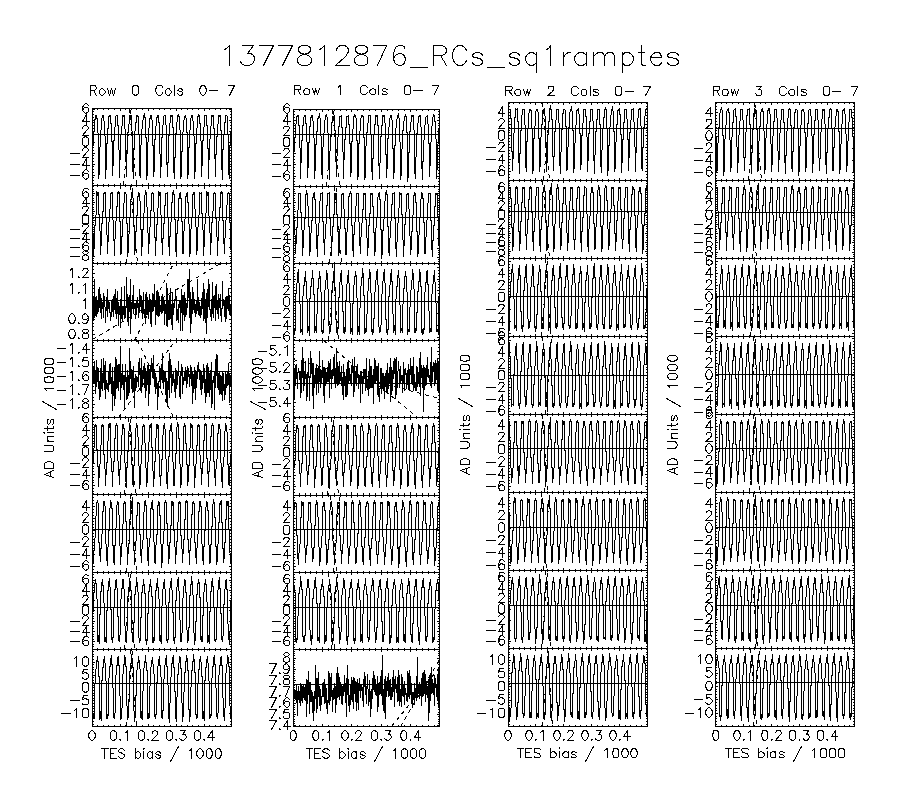
\includegraphics[width=\textwidth]{./images/1377812876_RCs_sq1ramptes_00.png}
\caption{Plot showing response of SQUID amplifier chain to a ramp in the \TES\ bias current, while \TES\ is superconducting.
  Data is shown for rows 0--4 for all eight columns.
  \RC{0}{2}, \RC{0}{3}, \RC{1}{3}, \RC{1}{7} all show no response, only noise (note the change in vertical scale for these row/columns).
  The vertical axis is in Analog-to-Digital-Converter units for the output of the \SQUID\ amplifier chain.
  The horizontal axis is the applied \TES\ bias current in \DAC\ units.
}
\label{fig:tes-bias-ramp-sc}
\end{figure*}

\begin{figure*}
\centering
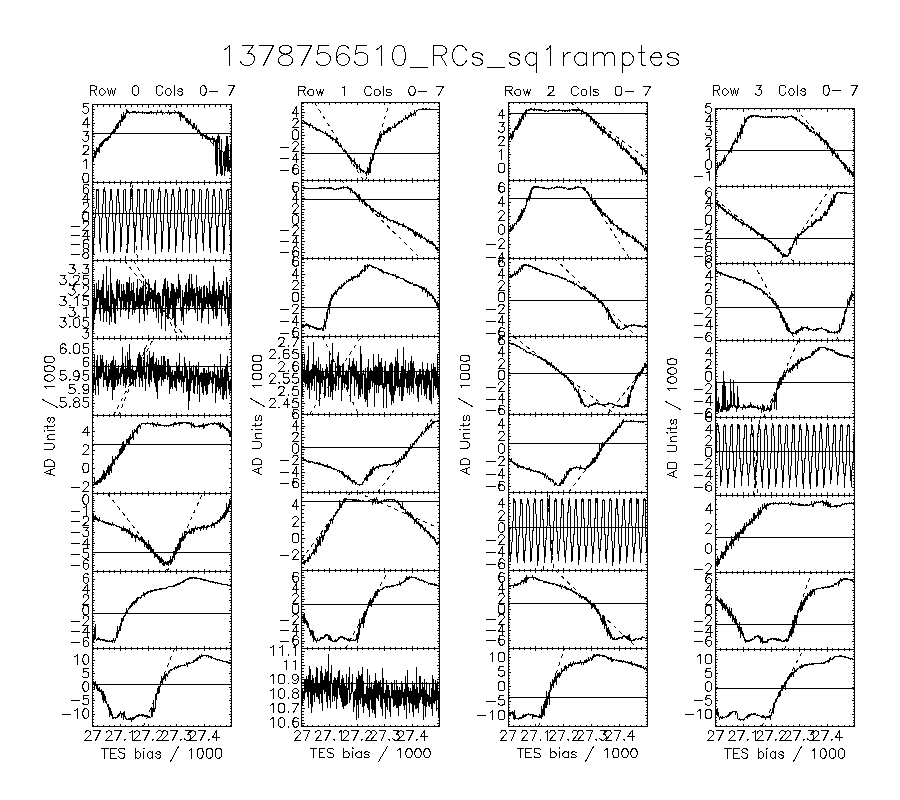
\includegraphics[width=\textwidth]{./images/1378756510_RCs_sq1ramptes_00.png}
\caption{Plot showing response of SQUID amplifier chain to ramp in \TES\ bias current, while \TES\ is biased into transition.
  The total change in applied bias current is the same as in \figref{fig:tes-bias-ramp-sc}.
  Data is shown for rows 0--4 for all eight columns.
  \RC{0}{2}, \RC{0}{3}, \RC{1}{3}, \RC{1}{7} all show no response, only noise (note the change in vertical scale for these row/columns).
  \RC{0}{1}, \RC{2}{5} and \RC{3}{4} all respond as if they were still superconducting (see \figref{fig:tes-bias-ramp-sc}).
  For the other detectors, the much slower mapping of the $V$-$\phi$ curve indicates a much higher resistance in the \TES\ circuit loop, due to the \TES\ sitting in the transition to the normal state.
  The axis units are the same as in \figref{fig:tes-bias-ramp-sc}.
}
\label{fig:tes-bias-ramp-trans}
\end{figure*}

\begin{figure*}
\centering
\includegraphics{./drawings/ch8-detector-cuts-wafer.pdf}
\caption{
Figure showing detector layout, highlighting which detectors have problems and which are working.
Each detector is labeled (below) with its row/column.
The x and y positions of the detectors on the wafer are also given in the format X-Y, where X give the x position of the detector (labeled along the bottom) and Y the y position (labeled along the left).
}
\label{fig:detector-cuts-wafer}
\end{figure*}

\begin{figure*}
\centering
\includegraphics{./drawings/ch8-detector-cuts-rc.pdf}
\caption{
  Figure showing same information as \figref{fig:detector-cuts-wafer}, but organized in term of readout rows/columns. Each detector is labeled (below) with its position on the detector wafer.
  The row/columns are labeled on the left and top. Unused row/columns as well as the row/columns used to readout the position of the secondary mirror are also indicated. }
\label{fig:detector-cuts-rc}
\end{figure*}

\section{Readout of Mirror Position}\label{sec:ch8-mirror-readout}

The \Imager\ produces a time-ordered data stream (``timestream'') containing the output of each detector as a function of time.
In order to turn this data stream into a video, we must know where the optical system is pointing at all times.
This section describes how this pointing information is placed directly into the timestream by the \Imager.
It is also necessary to know where each detector is pointed relative to the optical system; this relative detector pointing information is extracted from beam maps, as discussed in \sectionref{sec:ch8-beam-maps}.

The pointing of the optical system is set by the positions of the two \BOSE\ actuators --- \DISP1 and \DISP2 --- that move the secondary mirror%
\footnote{See \sectionref{sec:ch4-optical-design}}.
The actuator control hardware provides two voltage signal which are proportional to the positions of the actuators.
This voltage signal is sent into the \Imager\ cryostat by a pair coaxial cables.
Inside the cryostat two \SI{1}{m} long Phosphor Bronze \AWG36 twisted pair wires carry the signal to the focal plane, where the signal is fed into the input coil of a 1st stage \SQUID.
Series resistors (\SI{4.23}{\mega\ohm} for \DISP1, \SI{4.36}{\mega\ohm} for \DISP2) are used at room temperature to reduce the maximum current flowing through the wires to a value appropriate for the 1st stage \SQUID\ input; approximately \SI{2}{\uA}.

% Need add figure containing nice picture of the actuators/secondary
% from my talks

This approach synchronizes the actuator position readout with the detector response, and allows both pieces of information to be read out by the same warm and cold electronics.

To convert the mirror output current to actuator displacement I moved the mirror actuators in sine-wave patterns with a frequency of \SI{0.1}{\Hz} using 8 different displacement amplitudes.
I fitted the resulting output current timestream to sine waves.
The result are conversion factors of \SI{2.93}{\mm\per\uA} for \DISP1 and \SI{3.02}{\mm\per\uA} for \DISP2.
% see cooldown39/ana_bose_factor.m

To convert actuator displacement to displacements in the far-field of the system, I used the conversion factors list in \tableref{tab:ch4-zemax-parms}.
As discussed in \sectionref{sec:ch8-focus-distance}, although the system is configured to focus at \SI{16}{\m}, the actual focal distance is \SI{17}{\m}, so I used values for that distance from \tableref{tab:ch4-zemax-parms}.
A \SI{1}{\mm} movement of the actuator produces a rotation of the secondary mirror of \ang{0.276}; a \ang{1.0} rotation of the secondary mirror displaces the beam of an on-axis detector by \SI{19.33}{\cm} at the far-field focal plane.

To convert actuator displacements into locations in the far-field, three additional factors should be considered.
First, the Cassegrain optical system inverts images that it views, so that a beam from a detector in the lower left of the focal plane (as viewed from behind the detector focal plane) is pointed to the upper right on the far-field image (again as viewed from the system).
Second, tilting the mirror displaces the beams in the same direction as the mirror is tilted; this is easily seen by thinking of the system in transmission, and imagining the way a beam of light is reflected off of a rotated mirror).
Third, the actuators are oriented so that their rotation axes are rotated from horizontal/vertical by \ang{45}.
This all means that --- as viewed from the cryostat --- positive displacements of the \DISP1 actuator shift beams up and to the right, while positive displacements of the \DISP2 actuator shift beams up and to the left.
If we consider an $x$-$y$ coordinate system in the far-field, this means that the $x$ and $y$ displacement of the beams due to mirror movements are calculated as
\begin{equation}
\Delta x = F_d \frac{\sqrt{2}}{2} \left( I_{\text{DISP1}} \times \frac{\SI{2.93}{\mm}}{\SI{1}{\uA}} -
                              I_{\text{DISP2}} \times \frac{\SI{3.02}{\mm}}{\SI{1}{\uA}}  \right) \times
    \frac{\ang{0.276}} {\SI{1}{\mm}} \times
    \frac{\SI{19.33}{\cm}} {\ang{1}}
\end{equation}
\begin{equation}
\Delta y = F_d \frac{\sqrt{2}}{2} \left( I_{\text{DISP1}} \times \frac{\SI{2.93}{\mm}}{\SI{1}{\uA}} +
                              I_{\text{DISP2}} \times \frac{\SI{3.03}{\mm}}{\SI{1}{\uA}}  \right) \times
    \frac{\ang{0.276}} {\SI{1}{\mm}} \times
    \frac{\SI{19.33}{\cm}} {\ang{1}}
\end{equation}

Here I have also introduced a ``fudge factor'' $F_d$, which allows us to account for any error in manufacturing of the optics, errors in the \ZEMAX\ model, or errors in the \BOSE\ actuator control system; e.g., when we tell the \BOSE\ system to move an actuator by \SI{3}{\mm}, does it really move exactly \SI{3}{\mm}?
If none of these --- or other --- errors are present in the system, then $F_d$ will be equal to 1.0.
The direct measurements of distances in the far-field described in \sectionref{sec:ch8-dist-scale} show that $F_d = 1.098$, and this value is used in all analysis for the remainder of this chapter.

% pivot 14.19 mm behind mirror vertex
% pivot 14mm in front on \BOSE\ attachment point

A natural question is whether cross-talk appears between the actuator readout and the other detectors.
To test this both actuators were moved in a \SI{6}{\Hz} sine-wave pattern over their maximum displacement range of $\pm\SI{3.5}{\mm}$, while the detectors were biased at \SOC.
Both actuators were moved at the same time, roughly \SI{135}{\degree} out of phase.
The level of crosstalk present can be quantified by performing a least-squares fit of each detector timestream $\vect{d}_{rc}$ to the model
\begin{equation}
	 \vect{d}_{rc} = A_1 \vect{d}_{\text{DISP1}} + A_2 \vect{d}_{\text{DISP2}}.
\end{equation}
Here $\vect{d}_{\text{DISP1}}$ and $\vect{d}_{\text{DISP2}}$ are the measured outputs for each actuator.

The fit values for $A_1$ and $A_2$ were clustered about 0, and small compared to the noise in the detector timestream.
To check whether these small values were nevertheless real, I calculated the crosstalk amplitudes $A_1$ and $A_2$ for each detector twice: once of the first half of the data acquisition and once for the second half.
If crosstalk is present to a statistically significant level, a scatter plot of the crosstalk amplitudes for the two halves of the data acquisition should show signs of correlation.
As can be seen in \figref{fig:ch8-bose-cross}, the points are clustered about the origin and no correlation is apparent.

\begin{figure*}
\centering
\includegraphics{drawings/ch8-bose-cross.pdf}
\caption{
Plot showing crosstalk amplitudes.
The left plot is for \DISP1, the right for \DISP2.
Each actuator was moved +/- \SI{3.5}{\mm} at 6 Hz while the detectors were biased at \SOC.
The best-fit crosstalk amplitude for each actuator and detector were calculated for both the first half and the second half of the data acquisition, and these amplitudes are plotted against each other in these plots.
The lack of correlation in the scatter plots, as well as the clustering around the origin, indicate that any crosstalk present cannot be distinguished from noise in the detectors.
}
\label{fig:ch8-bose-cross}
\end{figure*}

\section{Focus Distance}\label{sec:ch8-focus-distance}

As described in \sectionref{sec:ch4-optical-design}, the \Imager\ is designed to focus at distances of \SIrange{16}{28}{\m}.
All results described in this chapter were with the \Imager\ configured to focus at 16~m.
To check the actual distance to the target focal plane, beam maps as described in \sectionref{sec:ch8-beam-maps} were performed with the black-body source located at different distance from the cryostat.
The optimal focus was a distance of \SI{17}{\m} from the apex of the primary mirror.
\figref{fig:ch8-focus} shows beam maps for the same detector taken at \SI{17}{\m} and at \SI{15.8}{\m}.
At \SI{17}{\m} the black-body aperture is well defined and much warmer than its surroundings.
At \SI{15.8}{\m}, the black-body aperture is visible, but poorly defined with significant side-lobes.
The temperature of the aperture is much closer to the background than in the \SI{17}{\m} case.

The reasons for the difference from \ZEMAX\ predictions are not understood.
Possibilities include the cryostat being located too close to the mirror system, or errors in the manufacturing or assembly of the optical components.

\begin{figure*}
\centering
\includegraphics{drawings/ch8-focus.pdf}
\caption{
  Plots showing impact of observing objects not located at the far-field focal plane.
  In both cases the \SI{1030}{\celsius} black-body source with aperture diameter set to \SI{0.4}{\in} (\SI{1.0}{\cm}) was observed. The acquisitions were taken 2.5\,minutes apart, and the only thing changed was the distance between the black-body and the primary mirror.
  \textbf{Left} Still image taken with the black-body located \SI{17}{\m} from the primary mirror.
  The aperture is clearly defined and \SI{80}{\K} warmer than its surroundings.
  % xxx need to comment on why 80 K is so much smaller than 1000 C
  \textbf{Right} Still image taken with the black-body located \SI{15.8}{\m} from the primary mirror.
  The black-body aperture is poorly defined with prominent side-lobe features.
  The aperture is no more than \SIrange{5}{10}{\K} warmer than the surroundings.
}
\label{fig:ch8-focus}
\end{figure*}

\section{Beam Maps} \label{sec:ch8-beam-maps}

As discussed in \sectionref{sec:ch4-feedhorn-design}, the \Imager\ feedhorns are predicted to have beams that are circularly symmetric and well-approximated by Gaussians with \FWHM\ of \SI{1.2}{\cm} at the target.
To verify these predictions beam maps were performed by rastering the beams over a stationary \SI{1030}{\celsius} black-body source.

The source used was an IR Labs IR-563/301\footnote{IRLabs, Inc. Tucson, AZ. USA} black-body.
This source reaches a maximum of \SI{1030}{\celsius} and has apertures ranging in size from \SIrange{0.0125}{0.6}{\in}.
Best results were achieved by covering an area around the black-body source with Aluminum foil; this eliminated hotspots in the image due to the warmth of the housing of the black-body source itself.
% xxx find this picture and add it! \figref{xxx} shows a picture of the black-body source with Aluminum foil mask.
The aperture diameter was set to \SI{0.2}{in} (\SI{0.51}{\cm}), which is small enough that the \FWHM\ of the resulting beam map will be larger than the beam map from a point source by an insignificant amount.

The \Imager\ beams were rastered over the black-body source by moving one actuator at \SI{6}{\hertz} while the other actuator moved much more slowly at \SI{0.1}{\hertz}.
Scans were taken with the black-body in two different locations to ensure coverage of the entire subarray.
At each black-body position two scans were taken with \DISP1 as the fast actuator and two with \DISP2 as the fast actuator, for a total of eight scans.

For each scan, the data stream for each detector was ``binned'' as described in \sectionref{sec:ch8-algo} to produce a beam map for each detector.
No common mode or polynomial was removed from the timestreams.
Actuator displacements were converted to distances in the far-field using the conversion factors discussed in \sectionref{sec:ch8-mirror-readout}.
The following 2-D Gaussian allowing for ellipticity was then fit to each beam map:
\begin{multline}
  % Note the use of the null delimiters \left. and \right. to allow
  % the equation to be broken over lines.
  P(x,y) = O + A \, \text{exp} \left[  - \frac{1}{2} \left( \frac{ (x-x_0) \cos{\theta} + (y-y_0) \sin{\theta}}{\sigma_1} \right)^2 \right. \\ 
                              \left. - \frac{1}{2} \left( \frac{-(x-x_0) \sin{\theta} + (y-y_0) \cos{\theta}}{\sigma_2} \right)^2
                       \right] .
\end{multline}
Here $x$ and $y$ represent the position in the beam map, while $x_0$, $y_0$, $\sigma_1$, $\sigma_2$, $\theta$, $A$, and $O$ are the parameters to be fit.
$O$ represents an overall \DC\ offset in the map level.
Only the points within \SI{3}{\cm} of the map peak were included in the fit.
Beam maps at the edge of the scan were discarded, as were beam maps where the fitting routine performed poorly. % xxx quantify
The $\theta$, $\sigma_1$, and $\sigma_2$ parameters were all rationalized so that the conditions $\sigma_1 > \sigma_2$ and $0 < \theta < \ang{180}$ hold.
The beam parameters across the eight scans were then averaged together to produce final beam maps.
\figref{fig:ch8-beam-summary} summarizes the final fit parameters for all the beams.
The beam ellipticity and angle offset from the $x$-axis are statistically significant.

\figref{fig:ch8-all-beam-maps} shows the final beam maps.
The beams are elliptical, with a mean $\sigma_1 / \sigma_2 = 1.6$.
The mean beam angle is $\ang{70}$ counter-clockwise from the $x$-axis.
The beam size \FWHM\ is \SI{1.4}{\cm}, and is calculated from
\begin{equation}
  2 \sqrt{2 \ln{2}} \sqrt{\sigma_1 \sigma_2}
\end{equation}
where the prefactor $2 \sqrt{2 \ln{2}}$ converts from the Gaussian parameters $\sigma_{i,2}$ to the \FWHM\ of the Gaussian.

In \sectionref{sec:ch4-feedhorn-design}, it was shown that the expected \FWHM\ beam width from this measurement is \SI{1.18}{\cm}, about \SI{19}{\percent} smaller than observed.
The beams should also be circular rather than strongly elliptical as observed.
The source of the large beams and ellipticity is not known, but three possible explanations are (1) misalignment of the feedhorns with the primary and secondary mirrors (2) diffraction off the aperture stop located in the \SI{50}{\kelvin} radiation shield (3) errors in fabrication of the mirrors or feedhorns.

The best-fit grid spacing between detector beams in the far field is \SI{1.98}{\cm}.
Using the plate scale extracted from \ZEMAX\ in \sectionref{sec:ch4-optical-design}, this is equivalent to a \SI{2.99}{\mm} detector spacing on the focal plane array.
The design detector spacing, after accounting for predicted thermal contraction of the feed-horn arrays, was \SI{2.730}{\mm}, \SI{8.6}{\percent} smaller than this.

To give a sense of the scale of the area covered directly by the beams relative to the field of view provided in images, \figref{fig:ch8-beams-on-image} shows the locations at which the beams are pointing when the \BOSE\ actuators are set to their zero positions.

Although the ellipticity of the beams is disappointing, the resolution is close to target, and the ellipticity is not a barrier to using the system to take video images.

\begin{figure*}
\centering
\includegraphics{drawings/ch8-beam-summary.pdf}
\caption{
  Plots summarizing final fit parameters for all beams.
  The histogram in the lower right shows that there is \abt{3} times more scatter in $\sigma_1$ than in $\sigma_2$. 
}
\label{fig:ch8-beam-summary}
\end{figure*}

\begin{figure*}
\centering
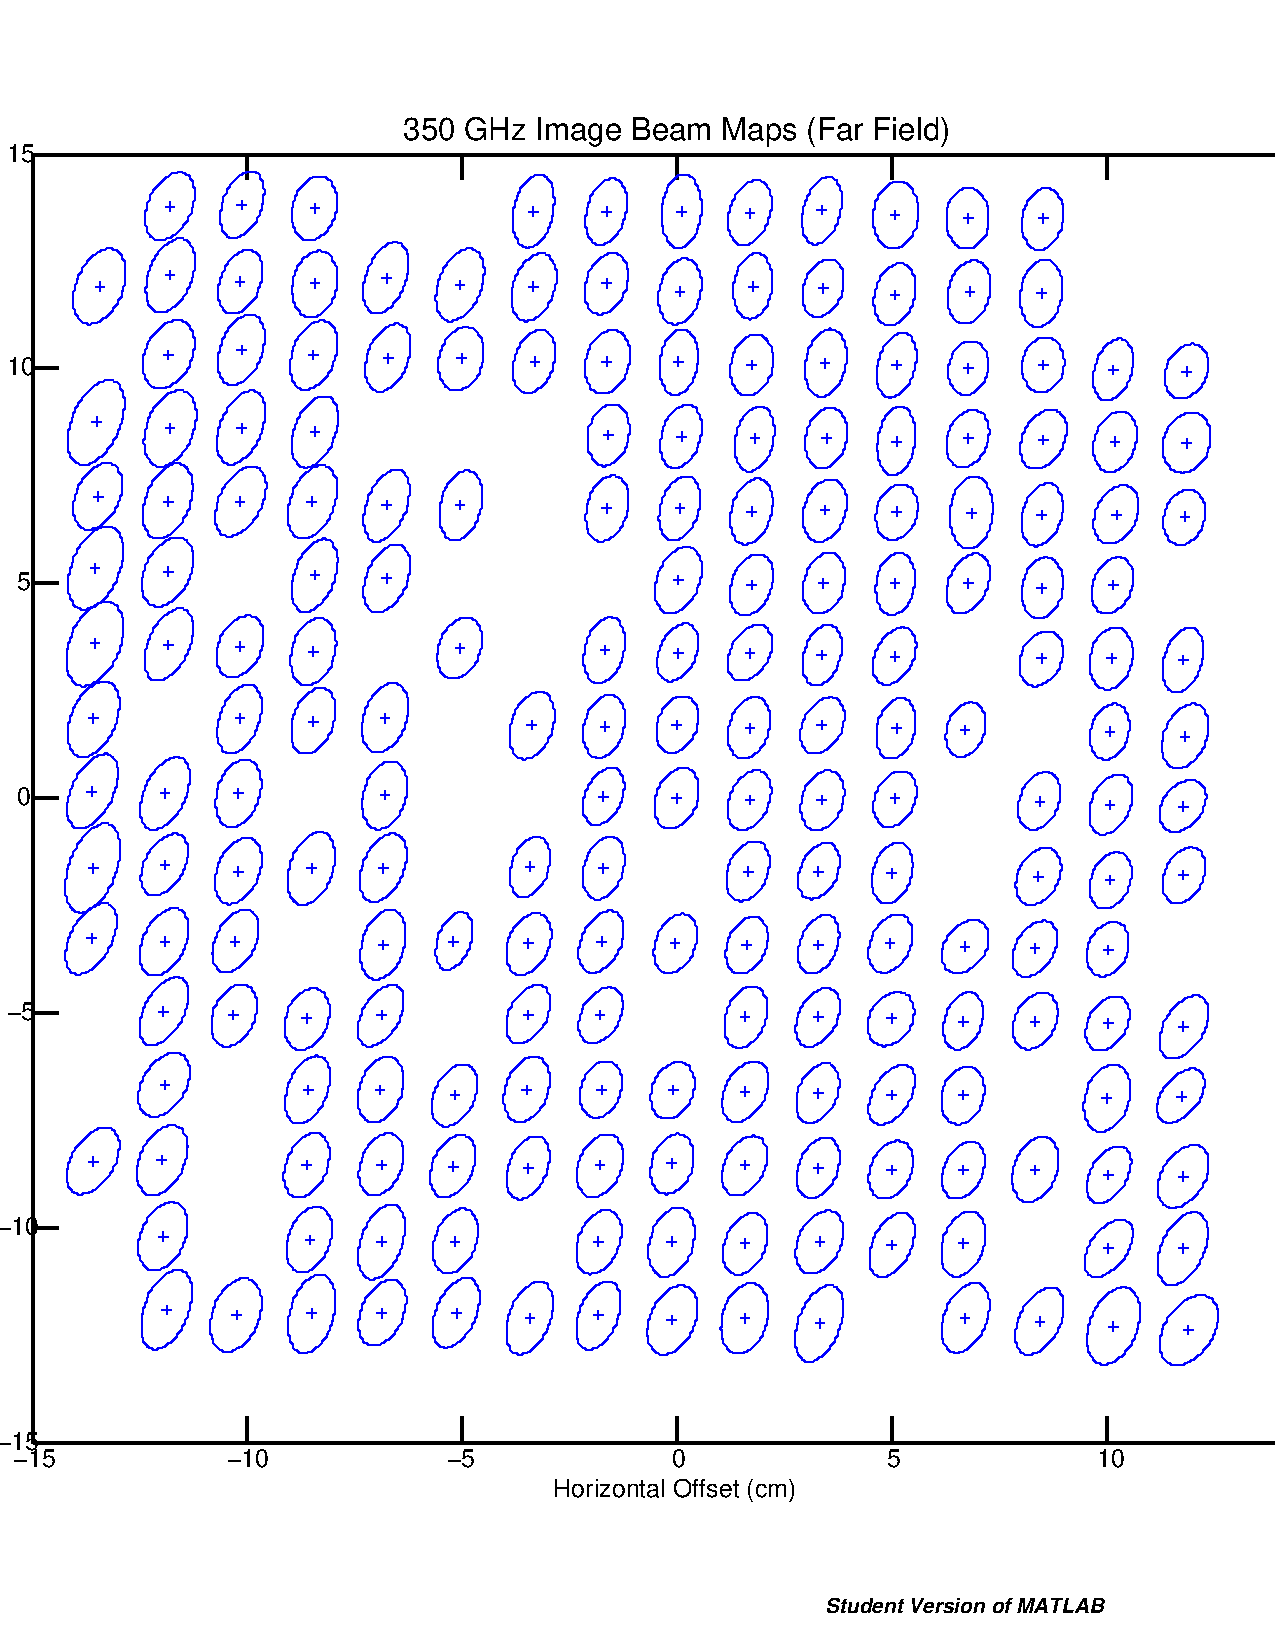
\includegraphics{drawings/ch8-all-beam-maps.pdf}
\caption{
Plot showing final beam maps.
The ellipses represent the full-width-half-maximum (\FWHM) of the best-fit 2-D Gaussian for each beam. The beams are elliptical, with a mean $\sigma_1/\sigma_2$ of 1.6, mean beam angle to the $x$-axis of \ang{70}, and beam \FWHM\ of \SI{1.4}{\cm}.
The four grid locations in the extreme upper right corner, as well as the extreme lower left grid point, have no detectors and therefore no beams. All other missing beams are for cut detectors, as discussed in \sectionref{sec:ch8-det-cuts}.
The offset is relative to detector \RCm{18}{4}.
}
\label{fig:ch8-all-beam-maps}
\end{figure*}

\section{Direct Measurement of Distance Scale and Image Resolution} \label{sec:ch8-dist-scale}

To measure the factor $F_d$ described in \sectionref{sec:ch8-mirror-readout}, I placed a Styrofoam cooler filled with liquid Nitrogen (LN2) in the far-field of the system and scanned the system over it, using data acquired to create still images.
A sheet of \ecco\footnote{Emerson \& Cuming Microwave Products, Inc.} was placed in the cooler to serve as a cold black surface for the system to observe.
Images were acquired of the cooler itself, as well as the cooler with aluminum foils strips taped to the outside.
Each strip was \abt{\SI{4}{\cm}} tall, and the strips were \SI{14.5}{\cm}, \SI{29}{\cm}, and \SI{47.2}{\cm} long.
The interior of the cooler is \SI{67.7}{\cm} wide.
For each image the \FWHM\ width of the strip --- or the cold space inside the cooler --- was calculated by taking a cut through the still image centered on the strip or cooler (see \figref{fig:ch8-check-dist}).

The result of these measurements is that $F_d = 1.098$.

\begin{figure*}
\centering
\includegraphics{drawings/ch8-check-dist.pdf}
\caption{
  Plots explaining measurement of distance scale.
  The left plot shows a close-up of the Styrofoam cooler filled with LN2, with an \SI{14.5}{\cm} by \SI{4}{\cm} strip taped to the outside.
  A cut of this image through the middle of strip (identified by the thin black line) is shown on the right.
  The \FWHM\ of this cut is shown as the red line.
  This measurement was repeated for two other Al foil strips, as well as the cooler without any Al foil strips, in order to establish the distance scale.
}
\label{fig:ch8-check-dist}
\end{figure*}

% Code: imaging/ana_reso_from_stills.m

Using the same cooler filled with LN2, a dime (diameter \SI{17.91}{\mm}) was taped to the outside of the cooler and a still image was taken.
\figref{fig:ch8-dime-map} shows the resulting still image, as well as a close-up of the are with the dime.
A 2-D Gaussian was fit to resulting map.
The best-fit Gaussian has ellipticity 1.16 --- smaller than the individual beams --- and the \FWHM\ of the dime map is \SI{2.0}{\cm} --- larger than the beams.
Both differences are expected from convolution of the beam with the dime, which is not a point source.
The \FWHM\ of the dime map is \SI{2.0}{\cm}; a bit larger than the dime's width of \SI{1.791}{\cm}, as expected due to convolution with the beam.
This serves as a rough confirmation of the beam size and locations as determined in \sectionref{sec:ch8-beam-maps}.

\begin{figure*}
\centering
\includegraphics{drawings/ch8-dime-map.pdf}
\caption{
  Plots showing still image of Styrofoam cooler filled with LN2, with a dime (diameter \SI{1.791}{\cm}) taped to it's outside.
  Red is warm, blue cold; the temperature scales are different in the two plots.
  \textbf{Left} The full map of the cooler. The white rectangle shows the area of the detail on the right.
  \textbf{Right} Detail of area within white rectangle: the dime.
  The black ellipse shows the \FWHM\ of the best-fit ellipse to the map. The ellipticity is \num{1.16}, the \FWHM\ of the principal axes are \SI{1.83}{\cm} and \SI{2.12}{\cm}, for an overall \FWHM\ of $\sqrt{1.83 \times 2.12} = \SI{2.0}{\cm}$.
}
\label{fig:ch8-dime-map}
\end{figure*}

\section{Optical Efficiency} \label{sec:ch8-opt-eff}

To measure the total optical efficiency of the system, \IV\ curves can be taken while a detector's beam is pointing at two known temperature distributions.
As discussed in \sectionref{sec:ch3-iv-curve}, the difference in Joule power at $0.99 R_n$ gives the difference in total power dissipated in the bolometer.
In this case, the power difference will be caused by the different amount of power absorbed in the bolometer while observing the two temperatures.
If the two temperatures are $T_1$ and $T_2$, then the total optical efficiency $\eta_{tot}$ is given by
\begin{equation}
  \eta_{tot} = \frac{P_{iv,1} - P_{iv,2}}{P_{opt}(T_2) - P_{opt}(T_2)},
\end{equation}
where $P_{IV}$ is the Joule power in the detector at $0.99 R_n$ and $P_{opt}(T)$ is the optical power in both polarizations emitted by the source in a single spatial mode, given by \eqnref{eqn:ch4-power-per-mode}.

For a good measurement the two temperatures $T_1$ and $T_2$ should be as far apart as possible, and the detector's far-field beam should be filled by the temperature distribution in each case.
I used the same ``\ecco\ submerged in LN2'' setup as described in \sectionref{sec:ch8-dist-scale} for the cold temperature.
For the warm temperature I used a sheet of \ecco\ backed by a thin sheet of Aluminum.
``Room Temperature'' here is assumed to be \SI{295}{\kelvin} (\SI{71.3}{\fahrenheit}).

Although the temperature of LN2 is well known to be \SI{77}{\kelvin}, this does not mean that the temperature seen by the beams when pointed at the cooler is exactly \SI{77}{\kelvin}.
\begin{itemize}
  \item The beams are looking through the \SI{1.625}{\in} thick Styrofoam walls of the cooler, which may have some emission themselves.
  \item Although the \ecco\ sunk in LN2 is opaque at \SI{350}{\GHz}, it may reflect some amount of light from the surrounding room.
  \item It is possible that a small amount of water vapor could condense on the outside of the cooler, leading to further emission.
\end{itemize}
For the purposes of this measurement I assumed that the cold \ecco\ was totally black and that no water vapor was condensed on the cooler, which is consistent with a visual examination.
However, I do allow for a non-unity transmittance $\tau$ for the Styrofoam in the analysis below.

For each of eight detectors, four IV curves were taken under three conditions: pointing at the room-temperature \ecco\ (``ecco''), pointing at the cold \ecco\ in the cooler (``LN2''), and looking at the \ecco\ with the cooler's lid placed directly in front of the cooler (``lid'').
The lid is \SI{2}{\in} thick and the cooler's side is \SI{1.625}{\in} thick.
I assume that the transmittance takes the form $e^{-d \kappa}$, where $d$ is the thickness of the material and $\kappa$ is some constant which characterizes the attenuation length of \SI{350}{\GHz} light in Styrofoam.
Given this assumption, if the transmittance through the cooler's wall is $\tau$, then the transmittance through the lid is given by $\tau^{2/1.625} = \tau^{1.23}$.

The optical powers viewed under these three conditions is then given by (with $T_h = \SI{295}{\K}$ and $T_c = \SI{77}{\K}$)
\begin{align}
  P_{opt,ecco}  & = P_{opt}(T_h) \\
  \begin{split}
    P_{opt,LN2} & = \tau P_{opt}(T_c) + (1-\tau)P_{opt}(T_h) \\
              & = P_{opt}(T_h) - \tau (P_{opt}(T_h) - P_{opt}(T_c)),
  \end{split} \\
  \begin{split}
    P_{opt,lid} & = \tau^{1.23} P_{opt,LN2} + (1-\tau^{1.23})P_{opt}(T_h) \\
              & = P_{opt}(T_h) - \tau^{2.23}(P_{opt}(T_h) - P_{opt}(T_c)) .
  \end{split}
\end{align}
Here these optical powers include both polarizations and are referred to power emitted at the target.
The differences in optical power absorbed in the bolometer will then be
\begin{align}
  \Delta P_{b,ecco-LN2} & = \eta_{tot} \tau (P_{opt}(T_h) - P_{opt}(T_c)) \\
  \Delta P_{b,lid-LN2}  & = \eta_{tot} \tau (1-\tau^{1.23}) (P_{opt}(T_h) - P_{opt}(T_c)).
\end{align}
These last two equations can be solved for $\eta_{tot}$ and $\tau$. The results are
\begin{equation}
   \tau = \sqrt[1.23]{1 - \frac{\Delta P_{b,lid-LN2}}{\Delta P_{b,ecco-LN2}}},
\end{equation}
\begin{equation}
   \eta_{tot} = \frac{\Delta P_{b,ecco-LN2}}{ \tau ( P_{opt}(T_h) - P_{opt}(T_c) )} .
\end{equation}

The full set of three IV curves were repeated three times over the course of several hours.
The transmittance $\tau$ of the cooler wall was found to be \abt{\SI{90}{\percent}} and the optical efficiency $\eta_{tot}$ was \SI{13.6}{\percent}. 
\tableref{tab:opt-eff} gives the results of these measurements averaged over all detectors and all repetitions.

This optical efficiency is roughly half of the value predicted in \sectionref{sec:ch4-opt-eff}.
It is not clear where the optical power is being lost.
\sectionref{sec:ch8-future-work} describes measurements that could help explain this problem.

\begin{table*}[t]
\centering
\caption{
Results of optical efficiency measurements.
The values are medians and the uncertainties give the \SIrange{25}{75}{\percent} range of measured values.
}
\label{tab:opt-eff}
\begin{tabular}{l l}
\toprule
Quantity &  Value \\
\midrule
$\eta_{tot}$ & $13.6 \pm  0.9$ \si{\percent} \\ 
$\tau$ & $90.6 \pm  4.8$ \si{\percent} \\ 
$P_{b,ecco-LN2}$   & $25.6 \pm  0.5$ \si{\pW} \\ 
$P_{b,lid-LN2}$ & $ 2.0 \pm  1.0$ \si{\pW} \\
\bottomrule
\end{tabular}
\end{table*}
 
\section{Establishment of Temperature Scale} \label{sec:ch8-temp-scale}

The output of the readout system gives changes in current passing through the detectors.
In order to convert this current change to a temperature change we must first convert the current changes to changes in power absorbed in the bolometer by dividing by the power-to-current responsivity $s_I$.
To convert this to temperature changes in the far-field of the system, we must use the total optical efficiency $\eta_{tot}$, as well as the Raleigh-Jeans limit of the optical power per spatial mode from a temperature distribution (see \sectionref{sec:ch4-opt-eff}).
The result is that the conversion from current to temperature is given by
\begin{equation} \label{eqn:ch8-I-to-T}
  \Delta T = \frac{\Delta I}{s_I(0) 2 k_B \eta_{tot} \Delta \nu}.
\end{equation}

Ideally this temperature scale would be measured directly by allowing the detectors to observe two known temperature distributions and measuring the resulting change in current.
However, this is easier said than done.
As the amount of optical power absorbed in a detector changes, the point occupied by the detector on its $R(T,I)$ surface changes, so that \Loop\, $\beta_I$, and the bias voltage $V_0$ all change.
This leads to a changing responsivity with optical load through \eqnref{eqn:si-full}.
For small changes in load (such as we expect in images taken with the system) the changes will be small and can be ignored.
But in order to obtain an accurate measurement of the temperature scale, it is desirable to use a large change in temperature, such as the difference between room temperature and LN2.
For these larger temperature changes the change in responsivity may not be negligible. 

To check the order of magnitude of this effect, I measured the detector responsivity directly using heaters both when the system was observing \ecco\ and when the cryostat window was covered with aluminum foil.
Covering the window with foil reduces the optical power reaching the detectors from outside the cryostat by \abt{\SI{38}{\pW}}.
For two of the detectors this lead to an increase in responsivity of \abt{\SI{1}{\percent}}, for the other two the increase was \abt{\SI{6.5}{\percent}}.
This makes using LN2 to establish a temperature scale that is more accurate than \abt{\SI{10}{\percent}} challenging.

Changing responsivity would not be a problem if the two temperatures were close to both each other and room temperature.
Stable, uniform temperature distributions using stirred liquid water are available \cite{dietlein_aqueous_2008} and should be used if a more accurate temperature mapping is desired in the future.

For this thesis, however, I have not made these measurements.
Instead I have assumed that all detectors have the same optical efficiency as was measured for eight detectors in \sectionref{sec:ch8-opt-eff}, $\eta_{tot} = 0.136$.
For $s_I(0)$ I have use the predicted values at \SOC\ of \sectionref{sec:bias-step}, with the exception of three detectors (\RCm{25}{4}, \RCm{26}{2}, \RCm{26}{4}) for which the predicted $s_I(0)$ was clearly incorrect, as judged from looking at detector timestreams and still images.
For these three images I have assumed a responsivity equal to the mean of all other predicted responsivities.

As a check on the accuracy of this temperature scale, the still image on the left of \figref{fig:ch8-dime-map} has \abt{\SI{180}{\K}} of contrast between the coldest section at the middle of the cooler and the warm area to the left of the cooler.
Given our estimate of transmittance $\tau$ of the cooler walls of \num{0.9}, the expected temperature differential is $0.9(295-77) = \SI{196}{\K}$.
Given the fact that responsivity will increase with optical loading, which leading to underestimates of temperature difference via \eqnref{eqn:ch8-I-to-T}, these numbers are fairly close.

From this I conclude that while the calibration temperature scale is likely not correct to within \SI{5}{\percent}, it is probably correct to within \SI{20}{\percent}.
Note that the uncertainty in this calibration does affect the noise in images produced by the system; it merely affects the number (\NETD) that we use to describe that noise.

\section{Image Processing Algorithm} \label{sec:ch8-algo}

This section describes the algorithm used to turn raw detector timestreams into video images.
The algorithm currently used is simple, processing each video frame independently.

The algorithm's steps are as follows:
\begin{enumerate}
\item The  \MCE\ channels containing the actuator displacement (\RCm{32}{5} for \DISP1 and \RCm{32}{6} for \DISP2) are converted to displacements in the far-field as described in \sectionref{sec:ch8-mirror-readout}.
\item Determine full range of far-field positions pointed to, accounting for all detectors. Define a \SI{1}{\cm} grid that covers this range in both $x$ and $y$ directions.
\item Each detectors output is multiplied by its ``current-to-temperature'' conversion factor (see \sectionref{sec:ch8-temp-scale}). At this point the units for all detector timestreams should be the same, but each detector timestream will have some unknown offset.
\item Divide detector timestreams into sections for each video frame based on \MCE\ readout rate and frequency at which the secondary mirror is rotating.
  If the mirror frequency is $f_m$ and the readout frequency is $f_{ro}$, then each video frame will cover $\lceil f_{ro} / f_{m} \rceil$ samples.
  \textbf{Example:} If the readout frequency is \SI{3125}{\Hz} and the mirror frequency is \SI{6}{\Hz}, then each video frame will cover $\lceil\frac{3125}{6}\rceil = \lceil 520.83 \rceil = 521$ samples.
\item For each video frame
  \begin{enumerate}
  \item Perform the following processing for each detector that is not on the cut list described in \sectionref{sec:ch8-det-cuts}:
    \begin{enumerate}
    \item If the detector's timestream shows evidence of glitches, do not include that detector's timestream for this video frame. The algorithm used to identify glitches is the following:
      \begin{enumerate}
      \item Calculate the differences $\Delta f_j = f_{j+1} - f_j$ between each consecutive value in the timestream.
      \item Calculate the standard deviation of the differences $\Delta f_j$.
      \item If the absolute value of any $\Delta f_j$ is greater than five times the standard deviation, identify this detector as having a glitch, so that it will be ignored for this video frame.
            On average this affects 3.2 detectors per frame.
            % xxx show example of glitch timestream? ... maybe show a big plot with all timestreams for a frame, highlighting those with glitches?
      \end{enumerate}
    \item Subtract the median value of this detector's timestream for this video frame.
          See the commentary below for a discussion of this approach to removing the detector offsets.
    \item If the detector does not have a glitch, determine which image pixel the detector is pointing to at each point in time, using both the pointing position from the actuator readout described in \sectionref{sec:ch8-mirror-readout} and the beam pointing information from \sectionref{sec:ch8-beam-maps}.
    \item Add the detector's value to that pixel for the frame.
    \item Keep track of the total number of samples that have been added to each pixel.
    \end{enumerate}
  \item After each detector has been processed for the frame, divide the total value for each pixel by the number of samples across all detectors that have been used for that pixel.
  \end{enumerate}
  \item To improve contrast, prior to presenting the images for display, map all temperature offset values below \SI{-3}{\K} to \SI{-3}{\K}, and all temperature values above \SI{3}{\K} to \SI{3}{\K}.
        Any pixels in the image with no data were assigned a temperature of \SI{-3}{\K}.
  \item After all video frames have been processed, convert the resulting 3-dimensional array to a video using \MATLAB's \texttt{VideoWriter} object.
\end{enumerate}

\subsection{Commentary on Videos Taken With the \Imager}

\figref{fig:ch8-single-frames} shows four still images from a video that was processed according to these rules.
This video can be viewed online at \url{http://www.youtube.com/watch?v=ul_fd-KWH38}. % fix this use correct URL for this particular video!
They show the author with a ceramic knife hidden beneath a button-down cotton shirt.
The ceramic knife is visible as a dark area on the left of the shirt.
A darker line running down the center of the shirt is due to the extra layer of cotton backing the buttons; this additional cloth produces more attenuation of the warm light from the body, and so appears cooler.

The total temperature contrast in the images of \figref{fig:ch8-single-frames} is \SI{6}{\K}, but as described above higher and low values of temperature have been mapped to \SI{+3}{\K} and \SI{-3}{\K} to improve contrast.
In the raw images, the mean total contrast across all frames with the person present is \SI{8.2}{\K}.

To estimate the expected contrast we can take the following into account:
\begin{itemize}
  \item Human skin temperature is typically in the range \SIrange{33}{35}{\celsius} = \SIrange{306.2}{308.2}{\K} \cite{ramanathan_new_1964}.
  \item The emissivity of human skin has been reported as \num{0.65} at \SI{100}{\GHz} and \num{0.93} at \SI{500}{\GHz} \cite{appleby_standoff_2007}.
        Interpolating between these values leads to an emissivity of \num{0.825} at \SI{350}{\GHz}.
  \item The temperature the room in which theses images were taken was \abt{\SI{295}{\K}}.
\end{itemize}
If the coldest temperature in the images is given by the room temperature, then the total contrast in the image is predicted as
\begin{equation} \label{eqn:ch8-pred-contrast}
  0.825 \times \SI{307}{\K} + (1 - 0.825) \times \SI{295}{\K} - \SI{295}{\K} =  \SI{9.9}{\K}.
\end{equation}
This is \SI{1.7}{\K} larger than observed.
Given uncertainties in the actual skin temperature of the person in the image, the true emissivity of human skin at \SI{350}{\GHz}, the true background temperature and the true temperature of the illuminating light, the closeness of the predicted and observed values gives confidence that our temperature scale is roughly correct.

\begin{figure*}
\centering
\includegraphics{drawings/ch8-single-frames.pdf}
\caption{
Sample still images from a video taken with the \Imager.
Time proceeds left-to-right and top-to-bottom.
The stills are 20 frames (\SI{3.33}{\s}) apart.
The person in the images is the author.
A ceramic knife hidden beneath a button-down cotton shirt is visible on the left of each image.
The darker line running down the center of the shirt is due to the extra layer of cotton backing the buttons; this additional cloth produces more attenuation of the warm light from the body.
As discussed in the text, the temperature range in these images was clipped to $\pm \SI{3}{\K}$ for better contrast.
The total contrast in the raw images is \SI{8.2}{\K}, about \SI{1.7}{\K} lower than expected.
See text for discussion.
}
\label{fig:ch8-single-frames}
\end{figure*}

\begin{figure*}
\centering
\includegraphics{drawings/ch8-beams-on-image.pdf}
\caption{
  Plot showing where beams are pointed in far-field.
  The background image is frame 25 from the video discussed in \sectionref{sec:ch8-algo}.
  The beam \FWHM\ ellipses are in blue.
}
\label{fig:ch8-beams-on-image}
\end{figure*}

\subsection{Commentary on Median-Subtraction}

As discussed in \sectionref{sec:det-readout}, the output of the readout system does not give the absolute current passing through each detector.
Instead it gives the change in current relative to some offset; an offset which is not a-priori known.
My approach for dealing with this offset is, for each video frame, to subtract from each detector's timestream the median of that detector's timestream during that video frame.
Although crude, this approach does a good job of accounting for the offsets in the detector timestreams, as well as accounting for the common-mode drift described in \sectionref{sec:ch7-common}.
However, elliptical scanning artifacts are still visible in the images of \figref{fig:ch8-single-frames}.
These artifacts arise in part because the median-subtraction scheme will work ``perfectly'' only in the case where the median temperature viewed by each detector during the frame is the same.
If this is not true for a particular detector, then ellipse traced out by that detector in the image will appear warmer or cooler than its surroundings (depending whether the distribution that it viewed was cooler or warmer than its surroundings), leading to elliptical scanning artifacts.

An additional consequence of this approach is that the median color in each video frame will be the same; i.e., a particular color in frame 1 may not represent the same temperature in frame 10.
This effect can be see in the early frames of the video available online.
In that video the early frames of the image are looking at the background of the lab, and only later does a person move into the frame.
As the person moves into the frame, some areas of the background become darker, not because they are changing to a lower temperature, but because they are now lower relative to the median temperature in the frame.
Although surprising when first seen, this effect does not prevent the system from being effective in detecting concealed weapons.

Other image processing algorithms could be used to better deal with the detector offsets.
One idea is to take a ``flat'' image of a uniform temperature distribution prior to taking videos, and use this image to normalize all detector offsets relative to each other.
However, a method would still be needed to deal with common-mode drift, as well as other sources of low-frequency $1/f$ noise which could cause detector offsets to drift independently of each other.

Another idea is to use the fact that the ellipse mapped out by each detector during a video frame overlaps with the ellipses of many other detectors.
It should be possible to take advantage of this to set the offsets for each detector correctly on a frame-by-frame basis.
It is possible that an approach like this could also be used to normalize the responsivity of all the detectors relative to each other.

An iterative approach is also possible, based on the fact that median-subtraction evidently comes close to perfectly removing detector offsets.
An algorithm could be developed which checks whether the points mapped out by each detector's ellipse are different than the neighboring points.
If the difference crosses some threshold, the offset could be adjusted and the frame processed with a new set of offsets.
This process could be repeated until a self-consistent image is created.

Other algorithmic approaches are certainly possible as well, and should be a focus of future work.

\section{Image Noise Model}\label{sec:ch8-noise-model}


The temperature scale established in \sectionref{sec:ch8-temp-scale} allows us to convert the measured detector white-noise level of \abt{\Pnoise{2.4e-15}} to a temperature noise via
\begin{equation}
  S_T = \frac{S_P(0)}{2 k_B \eta_{tot} \Delta \nu}.
\end{equation}
This results in a temperature noise level of \abt{\Tnoise{15e-3}}, referred to the temperature viewed in the far-field of the system.

To use this noise level to make a prediction for the \NETD\ in the image we can use the radiometer equation \cite{kraus_radio_1986}:
\begin{equation} \label{eqn:ch8-radiometer}
  \text{\NETD} = \frac{S_T}{\sqrt{2 t_{dwell}}},
\end{equation}
where $t_{dwell}$ is the total integration time including all detectors for each pixel in the image%
\footnote{%
In this equation the factor of 2 accounts for the fact that the noise power spectral density is defined so that the total variance in the signal is given by the integral of the power spectral density up to the one-half of the sampling frequency, i.e. up to the Nyquist frequency.
}.

All images in this chapter contain \abt{4030} pixels, each \SI{1}{\cm^2} in area%
\footnote{
  Although the images shown are all rectangular, due to the elliptical scanning pattern the actual area of the images that contains data is smaller than the rectangle.
}.
Each video frame lasts $\frac{1}{6}$\,\si{\s}, and there are \abt{210} good detector contributing.
$t_{dwell}$ is thus given by
\begin{equation} \label{eqn:ch8-t-dwell}
  t_{dwell} = \frac{210 \times \frac{1}{6}\,\si{s}}{4030} = \SI{8.7}{\ms}.
\end{equation}
Plugging this into \eqnref{eqn:ch8-radiometer} gives an \NETD\ of \abt{\SI{115}{\mK}}.

Verifying this noise level in a video image is difficult because we do not know a-priori whether there are any regions in the image which have a flat temperature distribution.
However, if we place a sheet of \ecco\ directly in front of the cryostat window, where all detector beams are large and covering similar areas, then all detectors should be viewing close to the same temperature distribution.
If data is acquired in this state, while the secondary mirror is moving, and the resulting timestreams are run through the same software used to create ``real'' videos, then the standard deviation of the temperature in each frame should give a good estimate of the \NETD.

I carried out this procedure, creating a ``flat'' video with 19 frames.
The mean \NETD\ across the 19 frames is \SI{101}{\mK}.
\figref{fig:ch8-flat-netd} shows a histogram of the \NETD\ distribution from all 19 frames, a histogram showing the temperature offset distribution for the second frame (which has $\NETD\ = \SI{100}{\mK}$), the second frame itself, and one of the still images from \figref{fig:ch8-single-frames}.
Both still images use the same temperature-difference-to-gray-scale mapping.

Comparing the two frames visually, it is clear that \NETD\ in the true video frame is dominated not by detector noise, but by artifacts of the scan, visible as elliptical arcs in the image.
These artifacts are likely caused by the median-subtraction scheme of \sectionref{sec:ch8-algo} not properly accounting for the detector offsets.
Nevertheless, in areas of the video still where there appear to be few scan artifacts (such as the arm on the lower right), the level of noise in the video still appears comparable to the flat still, indicating that \SI{100}{\mK} is a reasonable estimate of the \NETD\ in the image caused by detector noise.

\begin{figure*}
\centering
\includegraphics{drawings/ch8-flat-netd.pdf}
\caption{
  Plots relating to measurement of \NETD\ in flat frame images.
  \textbf{Upper Left} Histogram of \NETD\ for each of 19 frames taken from a ``flat'' video image. This \NETD\ is defined as the standard deviation of the temperatures across all pixels which were visited by at least one detector. 
  \textbf{Upper Right} Histogram showing distribution of temperature offsets within the second video frame, which has an \NETD\ of \SI{100}{\mK}.
                       The far left and far right bins include outliers that extend all the way to \SI{-1}{\K} on the left and \SI{1.5}{\K} on the right.
                       Removing these outliers results in \NETD\ values that are roughly \SI{15}{\percent} smaller.
  \textbf{Lower Left} The second frame of the flat video.
  \textbf{Lower Right} Frame 25 of the video discussed is \sectionref{sec:ch8-algo}.
These two frames use the same temperature-offset-to-color mapping to aid in visual comparison.
}
\label{fig:ch8-flat-netd}
\end{figure*}

The agreement between the predicted \NETD\ of \SI{115}{\mK} and the observed flat image \NETD\ of \SI{100}{\mK} is an encouraging sign that we understand the behavior of the system.
However, there are several ways in which the noise modeling used in this section simplifies matters:
\begin{itemize}
\item The white noise level for each detector is different.
\item The total integration time per pixel is not uniform.
      Some pixels end up receiving more detector samples then others, as shown in \figref{fig:ch8-flat-frame-cnt}.
\item The detector noise is not white.
      \eqnref{eqn:ch8-radiometer} is strictly only true for a noise spectrum that is white, while the detector noise spectrums have roll-offs due to the detector time constant $\tau_{eff}$, \SQUID\ noise, a roll-off due to the \SQUID\ servo loop, and other features.
      Because the noise roll-offs reduce the variance of the detector timestream, this should tend to reduce noise in the map.
      However, the roll-offs also mean that consecutive samples in a detector timestream are correlated, so that averaging them will not reduce noise by the full ``square-root of the number of samples'' factor that is appropriate for uncorrelated noise.
\end{itemize}
A more careful analysis of these factors would be useful, but has not yet been performed.

\begin{figure*}
\centering
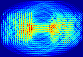
\includegraphics{drawings/ch8-flat-frame-cnt.pdf}
\caption{
  Distribution of samples per pixel for flat field image shown in \figref{fig:ch8-flat-netd}.
  Different video frames have slightly different distributions, but the overall features are all similar to what is shown here.
  The bins in the histogram on the right are one sample wide, so that it can be seen that a handful of pixels around the outer edge receive only one sample.
}
\label{fig:ch8-flat-frame-cnt}
\end{figure*}

\section{Directions for Future Work} \label{sec:ch8-future-work}

xxx need to write this section!
% xxx could a partial explanation for optical efficiency be the
% Piesiewicz alpha = 0.11 for HDPE? Would kill efficiency by factor of
% 0.88 relative to Lamb.

\begin{itemize}
\item better cryostat/mirror alignment
\end{itemize}
